% Created by tikzDevice version 0.12.6 on 2025-10-06 15:09:30
% !TEX encoding = UTF-8 Unicode
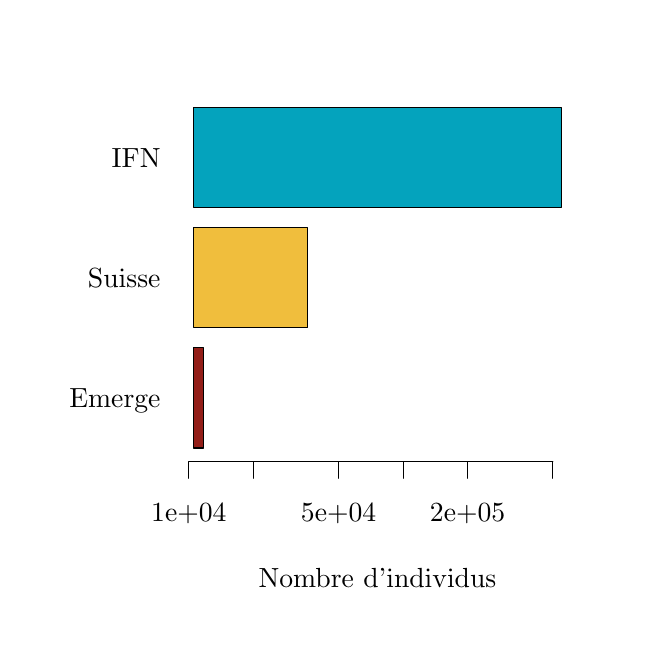
\begin{tikzpicture}[x=1pt,y=1pt]
\definecolor{fillColor}{RGB}{255,255,255}
\path[use as bounding box,fill=fillColor,fill opacity=0.00] (0,0) rectangle (216.81,216.81);
\begin{scope}
\path[clip] (  0.00,  0.00) rectangle (216.81,216.81);
\definecolor{drawColor}{RGB}{0,0,0}
\definecolor{fillColor}{RGB}{147,30,24}

\path[draw=drawColor,line width= 0.4pt,line join=round,line cap=round,fill=fillColor] ( 60.00, 64.92) rectangle ( 63.54,101.09);
\definecolor{fillColor}{RGB}{240,190,61}

\path[draw=drawColor,line width= 0.4pt,line join=round,line cap=round,fill=fillColor] ( 60.00,108.32) rectangle (101.25,144.49);
\definecolor{fillColor}{RGB}{4,163,189}

\path[draw=drawColor,line width= 0.4pt,line join=round,line cap=round,fill=fillColor] ( 60.00,151.72) rectangle (192.81,187.89);
\end{scope}
\begin{scope}
\path[clip] (  0.00,  0.00) rectangle (216.81,216.81);
\definecolor{drawColor}{RGB}{0,0,0}

\node[text=drawColor,anchor=base east,inner sep=0pt, outer sep=0pt, scale=  1.00] at ( 48.00, 79.56) {Emerge};

\node[text=drawColor,anchor=base east,inner sep=0pt, outer sep=0pt, scale=  1.00] at ( 48.00,122.96) {Suisse};

\node[text=drawColor,anchor=base east,inner sep=0pt, outer sep=0pt, scale=  1.00] at ( 48.00,166.36) {IFN};
\end{scope}
\begin{scope}
\path[clip] (  0.00,  0.00) rectangle (216.81,216.81);
\definecolor{drawColor}{RGB}{0,0,0}

\node[text=drawColor,anchor=base,inner sep=0pt, outer sep=0pt, scale=  1.00] at (126.41, 14.40) {Nombre d'individus};
\end{scope}
\begin{scope}
\path[clip] (  0.00,  0.00) rectangle (216.81,216.81);
\definecolor{drawColor}{RGB}{0,0,0}

\path[draw=drawColor,line width= 0.4pt,line join=round,line cap=round] ( 58.25, 60.00) -- (189.79, 60.00);

\path[draw=drawColor,line width= 0.4pt,line join=round,line cap=round] ( 58.25, 60.00) -- ( 58.25, 54.00);

\path[draw=drawColor,line width= 0.4pt,line join=round,line cap=round] ( 81.56, 60.00) -- ( 81.56, 54.00);

\path[draw=drawColor,line width= 0.4pt,line join=round,line cap=round] (112.37, 60.00) -- (112.37, 54.00);

\path[draw=drawColor,line width= 0.4pt,line join=round,line cap=round] (135.67, 60.00) -- (135.67, 54.00);

\path[draw=drawColor,line width= 0.4pt,line join=round,line cap=round] (158.98, 60.00) -- (158.98, 54.00);

\path[draw=drawColor,line width= 0.4pt,line join=round,line cap=round] (189.79, 60.00) -- (189.79, 54.00);

\node[text=drawColor,anchor=base,inner sep=0pt, outer sep=0pt, scale=  1.00] at ( 58.25, 38.40) {1e+04};

\node[text=drawColor,anchor=base,inner sep=0pt, outer sep=0pt, scale=  1.00] at (112.37, 38.40) {5e+04};

\node[text=drawColor,anchor=base,inner sep=0pt, outer sep=0pt, scale=  1.00] at (158.98, 38.40) {2e+05};
\end{scope}
\end{tikzpicture}
